% UTF-8 encoding
% Compile with latex+dvipdfmx, pdflatex, xelatex or lualatex

\documentclass[hyperref, UTF8]{ctexart}
\usepackage{amssymb}
\usepackage{amsmath}
\usepackage{graphicx}
\usepackage{subfigure}
\usepackage{geometry}
\usepackage{caption}
\usepackage{upgreek}
\newcommand{\under}[1]{\frac{1}{#1}}
\newcommand{\underpone}[1]{\frac{#1}{1+#1}}
\newcommand{\volt}{{\rm V}}
\newcommand{\source}{{\rm S}}
\newcommand{\second}{{\rm s}}
\newcommand{\ampere}{{\rm A}}
\newcommand{\milliampere}{{\rm mA}}
\newcommand{\microampere}{{\rm \upmu A}}
\newcommand{\hertz}{{\rm Hz}}
\newcommand{\ohm}{\Omega}
\newcommand{\kiloohm}{{\rm k}\Omega}
\newcommand{\watt}{{\rm W}}
\newcommand{\kilowatt}{{\rm kW}}
\newcommand{\degree}{^{\circ}}
\newcommand{\farad}{{\rm F}}
\newcommand{\microfarad}{{\rm \upmu F}}
\newcommand{\millifarad}{{\rm mF}}
\newcommand{\henry}{{\rm H}}
\newcommand{\J}{{\rm j}}
\newcommand{\D}{{\rm d}}
\newcommand{\E}{{\rm e}}

\title{电子学基础——第八次作业}
\author{LXQ}
\date{2019.11.27}

\geometry{left=2.0cm, right=2.0cm, top=2.5cm, bottom=2.5cm}
\linespread{1}

\begin{document}

\maketitle

\paragraph{6.38} \label{6.38}
    Construct the small-signal model of the circuits dipicted in Fig. 6-50. Assume all transistors operate in saturation and $\lambda \neq 0$

    \begin{figure}[!htb]
        \centering
        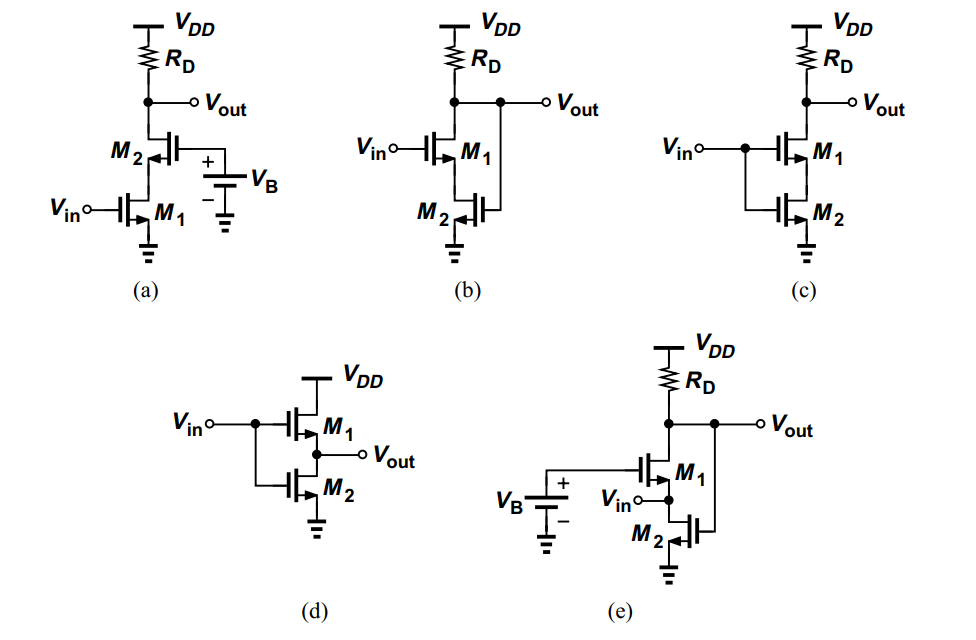
\includegraphics[width=0.651\textwidth]{p6-50.png}
        \caption*{Figure 6-50}
    \end{figure}    

\paragraph{解} 如图 p6-38 所示。

\newpage

    \begin{figure}[!htb]
        \centering
        \begin{minipage}[t]{0.409\textwidth}
        \centering
        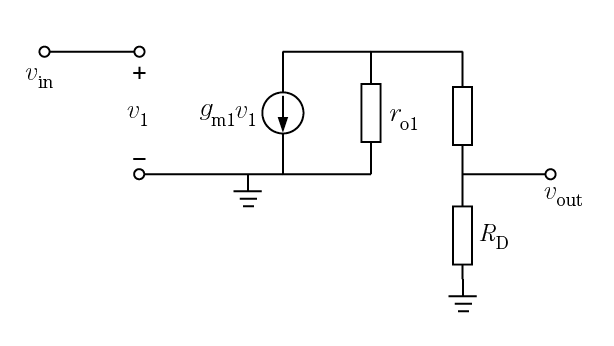
\includegraphics[width=1\textwidth]{p6-38-a-sol.png}
        \caption*{(a)}
        \end{minipage}
        \begin{minipage}[t]{0.463\textwidth}
        \centering
        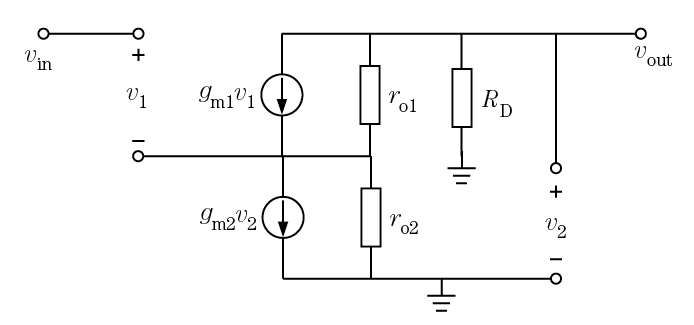
\includegraphics[width=1\textwidth]{p6-38-b-sol.png}
        \caption*{(b)}
        \end{minipage}
        \\
        \begin{minipage}[t]{0.397\textwidth}
        \centering
        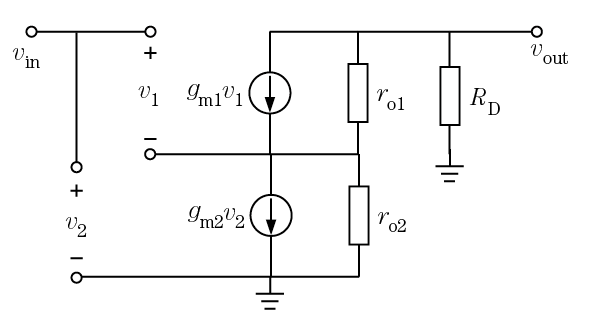
\includegraphics[width=1\textwidth]{p6-38-c-sol.png}
        \caption*{(c)}
        \end{minipage}
        \begin{minipage}[t]{0.347\textwidth}
        \centering
        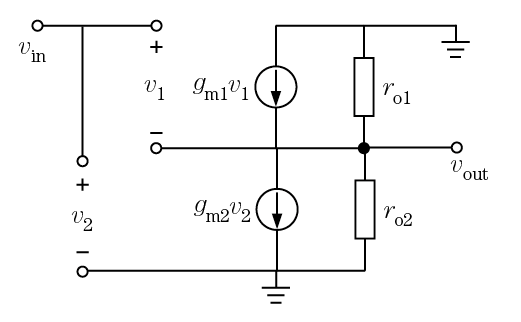
\includegraphics[width=1\textwidth]{p6-38-d-sol.png}
        \caption*{(d)}
        \end{minipage}
        \\
        \begin{minipage}[t]{0.485\textwidth}
        \centering
        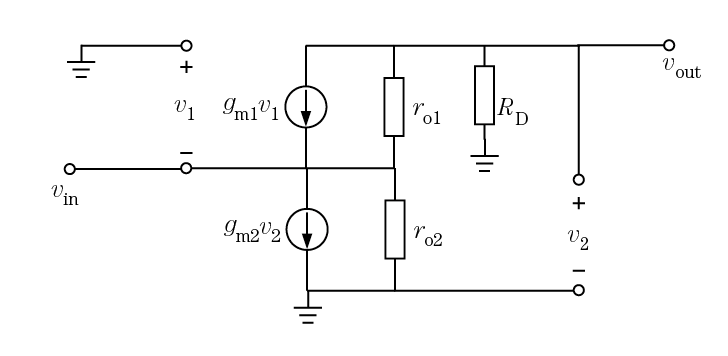
\includegraphics[width=1\textwidth]{p6-38-e-sol.png}
        \caption*{(e)}
        \end{minipage}
        \caption*{Figure p6-38}
    \end{figure}

\paragraph{6.46} \label{6.46}
    Consider the circuit depicted in Fig. 6-57, where $M_1$ and $M_2$ operate in saturation and exhibit channel-length modulation coefficients $\lambda_n$ and $\lambda_p$, respectively.

    \begin{figure}[!htb]
        \centering
        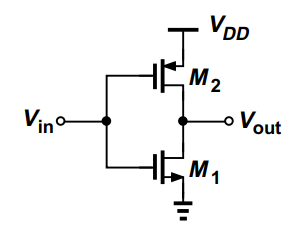
\includegraphics[width=0.203\textwidth]{p6-57.png}
        \caption*{Figure 6-57}
    \end{figure}    

    (a) Construct the small-signal equivalent circuit and explain why $M_1$ and $M_2$ appear in "parallel."

    (b) Determine the small-signal voltage gain of the circuit.

\paragraph{解}

    (a) 小信号电路图如图 p6-46 所示。由于两个MOSFET管的D端即$v_{out}$,而S端接地,从而在小信号电路中表现为并联。

    \begin{figure}[!htb]
        \centering
        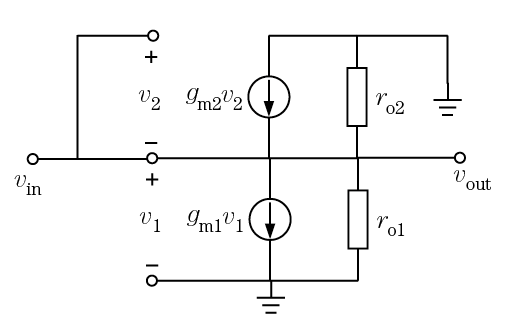
\includegraphics[width=0.343\textwidth]{p6-46-sol.png}
        \caption*{Figure p6-46}
    \end{figure}
    
    (b) 可列得以下方程

    \begin{gather*}
        \left\{ \begin{aligned}
            \frac{v_{out}}{r_{o1}}+\frac{v_{out}}{r_{o2}} & = g_{m2}v_2 + g_{m2}v_1 \\
            v_2 & = v_{in}-v_{out} \\
            v_1 & = v_{in}
        \end{aligned} \right.
    \end{gather*}
    $$\therefore A_v = \frac{v_{out}}{v_{in}} = \frac{g_{m1}+g_{m2}}{\frac{1}{r_{o1}}+\frac{1}{r_{o2}}+g_{m2}}$$

\paragraph{7.28} \label{7.28}
    If $\lambda \neq 0$, determine the voltage gain of the stages shown in Fig. 7-60. 

    \begin{figure}[!htb]
        \centering
        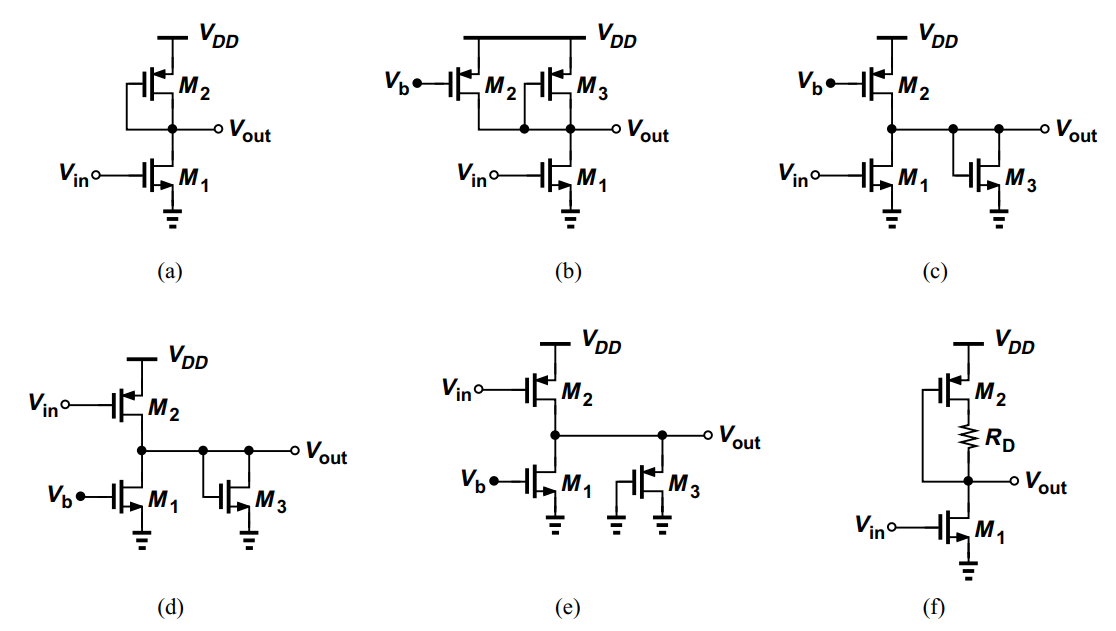
\includegraphics[width=0.744\textwidth]{p7-60.png}
        \caption*{Figure 7-60}
    \end{figure}
    
\paragraph{解}

    (a)$M_2$为二极管接法,可看作电阻$\frac{1}{g_m2}//r_{o2}$,则$M_1$为共源放大器,
    $$A_v = -g_{m1}(r_{o1}//r_{o2}//\frac{1}{g_m2})$$

    (b)$M_2$可视为$r_{o2}$,$M_3$为二极管接法,可视为$\under{g_{m3}}//r_{o3}$,则$M_1$为共源接法,
    $$A_v = -g_{m1}(r_{o1}//r_{o2}//r_{o3}//\under{g_{m3}})$$

    (c)$M_2$可视为$r_{o2}$,$M_3$为二极管接法,可视为$\under{g_{m3}}//r_{o3}$,则$M_1$为共源接法,
    $$A_v = -g_{m1}(r_{o1}//r_{o2}//r_{o3}//\under{g_{m3}})$$
    
    (d)$M_1$可视为$r_{o1}$,$M_3$可视为$\under{g_{m3}}//r_{o3}$,$M_2$为共源接法,
    $$A_v = -g_{m2}(r_{o2}//r_{o1}//r_{o3}//\under{g_{m3}})$$

    (e)$M_1$可视为$r_{o1}$,$M_3$D,G端接地,是为二极管接法,可视为$\under{g_{m3}}//r_{o3}$,$M_2$为共源放大器,
    $$A_v = -g_{m2}(r_{o2}//r_{o1}//r_{o3}//\under{g_{m3}})$$

    (f)首先考察从$M_1$的漏端向上看的输出电阻,其小信号电路如图 p7-28-f 所示。可设输入信号为$v$,产生$i$的电流。

    \begin{figure}[!htb]
        \centering
        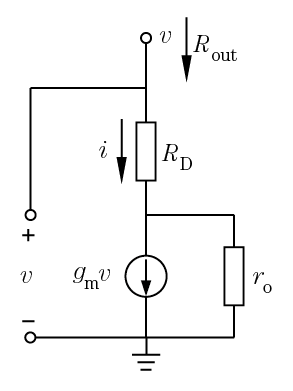
\includegraphics[width=0.195\textwidth]{p7-28-f-sol.png}
        \caption*{Figure p7-28-f}
    \end{figure}

    则$$iR_D + (i - vg_m) r_o = v$$
    $$\therefore R_{out}=\frac{v}{i}=\frac{R_D+r_o}{1+g_mr_o}$$
    从而$M_2$等效为$r_2=\frac{v}{i}=\frac{R_D+r_o}{1+g_mr_o}$,$M_1$为共源接法,则
    $$A_v = -g_{m1}(r_{o1}//r_2) = -g_{m1}(r_{o1}//\frac{R_D+r_o}{1+g_mr_o})$$

\paragraph{7.46}\label{7.46}
    Consider the circuit of Fig. 7-73, where a common-source stage ($M_1$ and $R_{D1}$) is followed by a common-gate stage ($M_2$ and $M_{D2}$).

    \begin{figure}[!htb]
        \centering
        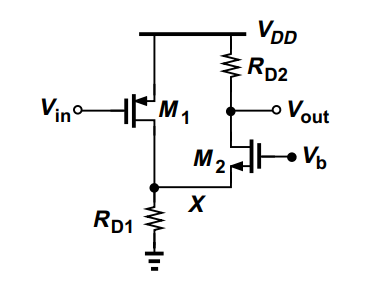
\includegraphics[width=0.249\textwidth]{p7-73.png}
        \caption*{Figure 7-73}
    \end{figure}
        
    (a) Writing $v_{out}/v_{in} = (v_X / v_{in})(v_{out}/v_X)$ and assuming $\lambda=0$, compute the overall voltage gain.

    (b) Simplify the result obtained in (a) if $R_{D1} \rightarrow \infty$. Explain why this result is to be expected.

\paragraph{解}

    (a) $M_1$放大器为共源放大器,负载$R_1=R_{D1}//\under{g_{m2}}$则
    $$\frac{v_x}{v_{in}}=-g_{m1}(R_{D1}//\under{g_{m2}})$$
    而$M_2$为共栅放大器,则
    $$\frac{v_{out}}{v_x}=g_{m2}R_{D2}$$
    从而$\frac{v_{out}}{v_{in}}=-g_{m1}g_{m2}R_{D2}(R_{D1}//\under{g_{m2}})$

    (b) $$R_{D1} \rightarrow \infty, \frac{v_{out}}{v_{in}} \rightarrow -g_{m1}R_{D2}$$
    $R_{D1} \rightarrow \infty$时,原电路中可视$R_{D1}$为断路,而$M_2$共栅,可视为导线,则原电路简化为仅有$M_1$作为共源放大器负载$R_{D2}$的电路,则$A_v = -g_{m1}R_{D2}$。

\paragraph{7.47} \label{7.47}
    Assuming $\lambda=0$, calculate the voltage gain of the circuit shown in Fig. 7-74. Explain why this stage is \emph{not} a common-gate amplifier. 

    \begin{figure}[!htb]
        \centering
        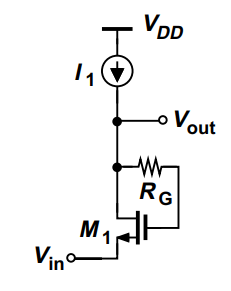
\includegraphics[width=0.154\textwidth]{p7-74.png}
        \caption*{Figure 7-74}
    \end{figure}

\paragraph{解} 小信号电路如图 p7-47 所示
    \begin{figure}[!htb]
        \centering
        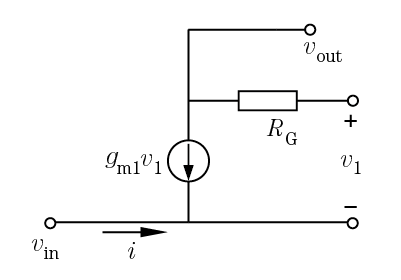
\includegraphics[width=0.267\textwidth]{p7-47-sol.png}
        \caption*{Figure p7-47}
    \end{figure}
    \begin{gather*}
        \left\{ \begin{aligned}
            v_{in}+v_1 & = v_{out} \\
            g_mv_1 & = 0 \\
        \end{aligned}\right.
    \end{gather*}
    $$\therefore v_{in}=v_{out}, A_v = 1$$

    该电路不是共栅放大器的原因是栅端和漏端并非直接相连而是通过电阻。
    
\paragraph{7.55}\label{7.55}
    Determine the voltage gain of the stages shown in Fig. 7-80. Assume $\lambda \neq 0$.

    \begin{figure}[!htb]
        \centering
        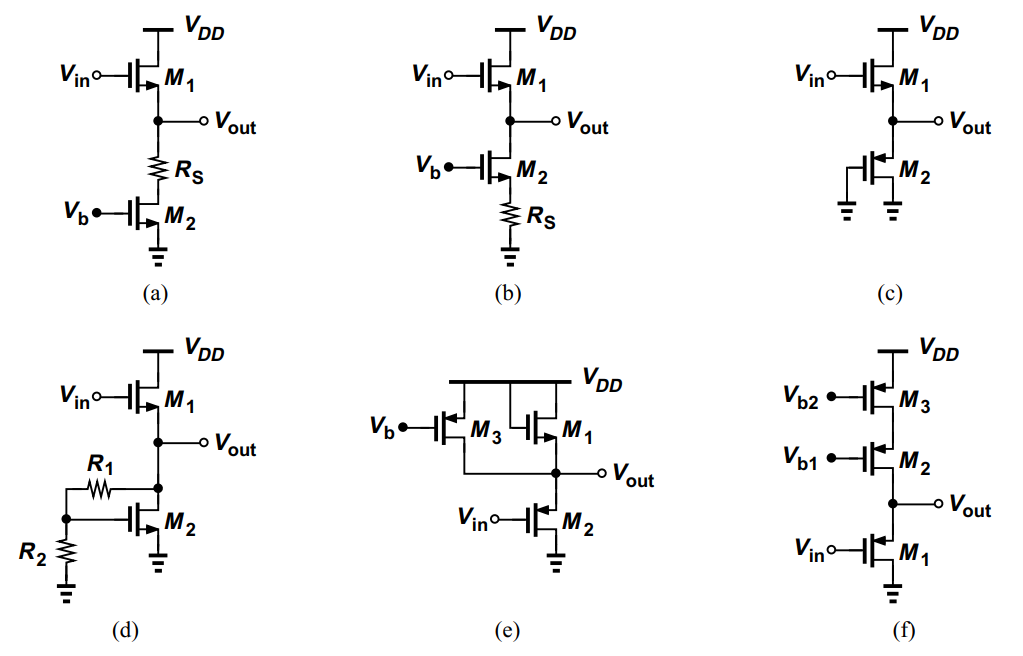
\includegraphics[width=0.682\textwidth]{p7-80.png}
        \caption*{Figure 7-80}
    \end{figure}

\paragraph{解}

    (a) $M_2$可视作$r_{o2}$,$M_1$为源极跟随器,则
    $$A_v = \frac{g_{m1}[r_{o1}//(R_S+r_{o2})]}{1+g_{m1}[r_{o1}//(R_S+r_{o2})]}$$

    (b) $M_2$与$R_S$构成源简并放大器,可等效为$(1+g_{m2}r_{o2})R_S+r_{o2}$,$M_1$为源极跟随器,则
    $$A_v = \underpone{g_{m1}[r_{o1}//((1+g_{m2}r_{o2})R_S+r_{o2})]}$$

    (c) $M_2$为二极管接法,等效于$\under{g_{m2}}//r_{o2}$,$M_1$为源极跟随器,则
    $$A_v = \underpone{g_{m1}(r_{o1}//\under{g_{m2}}//r_{o2})}$$

    (d) 可先求$v_{out}$以下部分的等效电阻$r_{out}$,小信号电路如图 p7-55-d 所示。
    \begin{figure}[!htb]
        \centering
        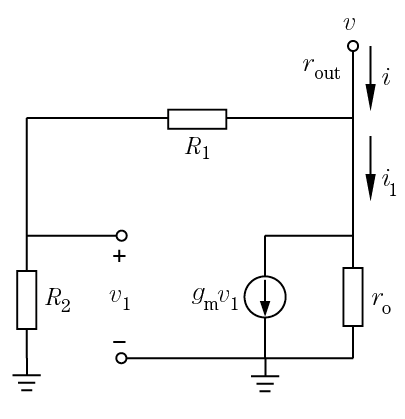
\includegraphics[width=0.270\textwidth]{p7-55-d-sol.png}
        \caption*{Figure 1}
    \end{figure}    
    \begin{gather*}
        \left\{ \begin{aligned}
            v &= [i_1-g_m(v-(i-i_1)R_1)]r_o \\
            v &= (i-i_1)(R_1+R_2)
        \end{aligned}\right.
    \end{gather*}
    $$\therefore r_{out}=\frac{v}{i}=\frac{r_o(R_1+R_2)}{R_1+R_2+r_o+g_mr_oR_2}$$
    
    而$M_1$为源极跟随器,从而
    $$A_v = \underpone{g_{m1}(r_{o1}//\frac{r_{o2}(R_1+R_2)}{R_1+R_2+r_{o2}+g_{m2}r_{o2}R_2})}$$
    
    (e) $M_3$可视作$r_{o3}$,$M_1$可视作$\under{g_{m1}}//r_{o1}$,$M_2$为源极跟随器,则
    $$A_v = \underpone{g_{m2}(r_{o2}//r_{o1}//r_{o3}//\under{g_{m1}})}$$

    (f) $M_2,M_3$可视为电阻$r=(1+g_{m2}r_{o2})r_{o3}+r_{o2}$,而$M_1$为源极跟随器,则
    $$A_v = \underpone{g_{m1}[r_{o1}//((1+g_{m2}r_{o2})r_{o3}+r_{o2})]}$$

\paragraph{7.56}\label{7.56}
    Consider the circuit of Fig. 7-81, where a source follower ($M_1$ and $I_{1}$) precedes a common-gate stage ($M_2$ and $M_{D}$).

    \begin{figure}[!htb]
        \centering
        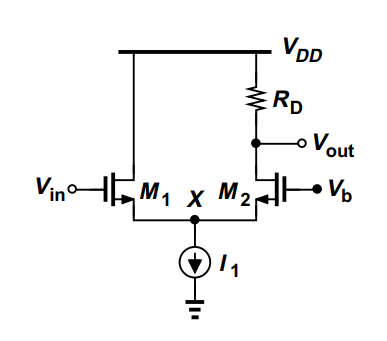
\includegraphics[width=0.258\textwidth]{p7-81.png}
        \caption*{Figure 7-81}
    \end{figure}    
        
    (a) Writing $v_{out}/v_{in} = (v_X / v_{in})(v_{out}/v_X)$, compute the overall voltage gain.

    (b) Simplify the result obtained in (a) if $g_{m1}=g_{m2}$. 

\paragraph{解}

    (a) $M_1$为源极跟随器,$R_L = R_{2in} = \under{g_{m2}}$
    $$\therefore \frac{v_x}{v_{in}}=\underpone{g_{m1}\cdot\under{g_{m2}}}=\frac{g_{m1}}{g_{m1}+g_{m2}}$$
    
    $M_2$为共栅放大器,则
    $$\frac{v_{out}}{v_x}=g_{m2}R_D$$
    $$\therefore \frac{v_{out}}{v_{in}}=\frac{g_{m1}g_{m2}R_D}{g_{m1}+g_{m2}}$$

    (b) $g_{m1}=g_{m2}=g_{m}$时
    $$\frac{v_{out}}{v_{in}}=\frac{g_mR_D}{2}$$
        
\paragraph{9.19} \label{9.19}
    Determine the output impedance of the stages shown in Fig. 9-52. Assume all of the transistors operate in saturation and $g_mr_O >> 1$. 

    \begin{figure}[!htb]
        \centering
        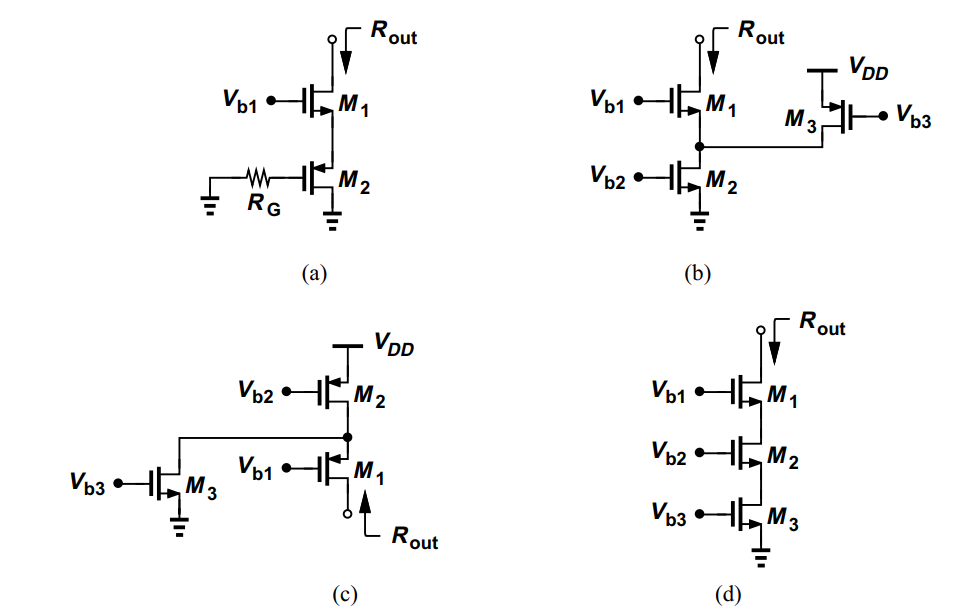
\includegraphics[width=0.640\textwidth]{p9-52.png}
        \caption*{Figure 9-52}
    \end{figure}

\paragraph{解}

    (a) $R_G$上无电流,则$M_2$为二极管接法,可视为$r=\under{g_{m2}}//r_{o2}$,而$M_1$为源简并放大器,则
    $$r_{out}=(1+g_{m1}r_{o1})(\under{g_{m2}}//r_{o2})+r_{o1} \approx r_{o1}(\frac{g_m1}{g_m2}+1)$$

    (b) $M_2,M_3$均共源,则可分别视为$r_{o2},r_{o3}$,而$M_1$为源简并放大器,则
    $$r_{out}=(1+g_{m1}r_{o1})(r_{o2}//r_{o3})+r_{o1} \approx g_{m1}r_{o1}(r_{o2}//r_{o3})+r_{o1}$$

    (c) $M_2,M_3$均共源,则可分别视为$r_{o2},r_{o3}$,而$M_1$为源简并放大器,则
    $$r_{out}=(1+g_{m1}r_{o1})(r_{o2}//r_{o3})+r_{o1} \approx g_{m1}r_{o1}(r_{o2}//r_{o3})+r_{o1}$$

    (d) $M_3$共源,可视为$r_{o3}$,$M_2$为源简并放大器,可视为
    $$r_2 = (1+g_{m2}r_{o2})r_{o3}+r_{o2} \approx g_{m2}r_{o2}r_{o3}$$

    $M_1$亦为源简并放大器,则
    $$r_{out}=(1+g_{m1}r_{o1})g_{m2}r_{o2}r_{o3}+r_{o1} \approx g_{m1}g_{m2}r_{o1}r_{o2}r_{o3}$$
    
\paragraph{9.32} \label{9.32}
    In the cascode stage of Fig. 9-20(b), $(W/L)_1=\cdots=(W/L)_4 = 20/0.18$. If $\mu_nC_{ox}=100\microampere/\volt^2$, and $\mu_pC_{ox}=50\microampere/\volt^2$, $\lambda_n = 0.1 \volt^{-1}$, and $\lambda_p=0.15\volt^{-1}$, calculate the bias current such that the circuit achieves a voltage gain of 500.

    \begin{figure}[!htb]
        \centering
        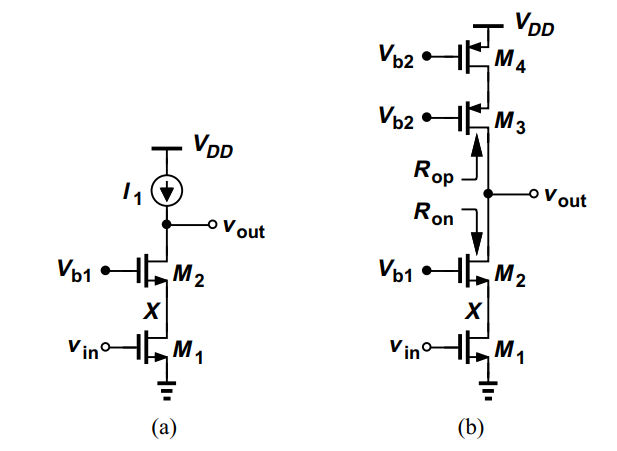
\includegraphics[width=0.411\textwidth]{p9-20.png}
        \caption*{Figure 9-20}
    \end{figure}

\paragraph{解} 
    \begin{align*}
        g_{m1}&=g_{m2} = \sqrt{2\mu_nC_{ox}(W/L)I_D}=149\sqrt{I_D} \\
        g_{m3}&=g_{m4} = \sqrt{2\mu_pC_{ox}(W/L)I_D}=105\sqrt{I_D} \\
        r_{o1}&=r_{o2} = \under{\lambda_nI_D} = \frac{10}{I_D} \\
        r_{o3}&=r_{o4} = \under{\lambda_pI_D} = \frac{6.67}{I_D} \\
        A_v & \approx -g_{m1}(((1+g_{m3}r_{o3})r_{o4}+r_{o3}) // ((1+g_{m2}r_{o2})r_{o1}+r_{o2})) \\
        & \approx -g_{m1}[(g_{m3}r_{o3}r_{o4})//(g_{m2}r_{o2}r_{o1})] \\
        & = -531400 / I_D
    \end{align*}
    上式中$I_D$以$\microampere$为单位。

    欲使增益达到500,则$I_D=1.06\milliampere$。

\paragraph{9.34} \label{9.34}
    Determine the voltage gain of each circuit in Fig. 9-59. Assume $g_mr_O>>1$.

    \begin{figure}[!htb]
        \centering
        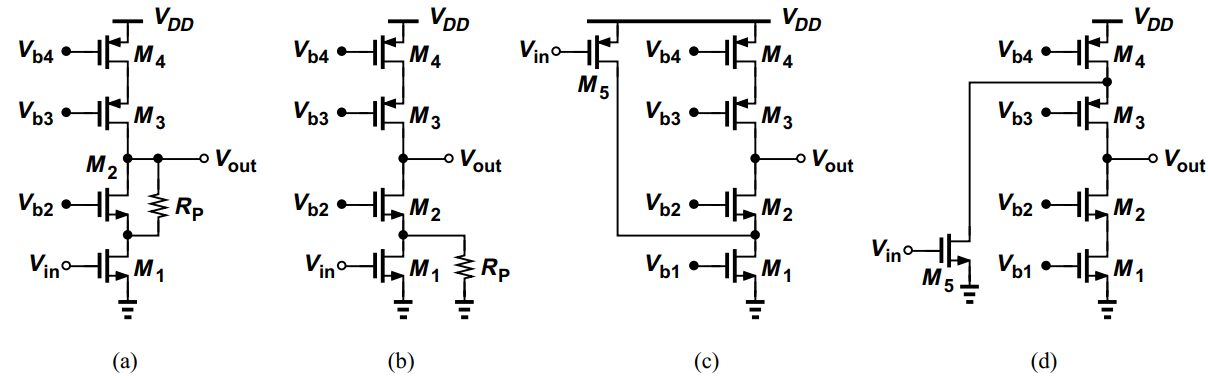
\includegraphics[width=0.805\textwidth]{p9-59.png}
        \caption*{Figure 9-59}
    \end{figure}

\paragraph{解}

    (a) \begin{align*}
        G_m &= g_{m1} \cdot \frac{r_{o1}}{r_{o1}+\under{g_{m2}//r_{o2}//R_P}} \\
        & \approx \frac{g_{m1}r_{o1}}{r_{o1}+\under{g_{m2}}//R_P} 
    \end{align*}
    \begin{align*}
        R_{out} &= [(1+g_{m3})r_{o4}+r_{o3}]//[(1+g_{m2}(r_{o2}//R_P))r_{o1}+r_{o2}//R_P] \\
        & \approx [g_{m3}r_{o3}r_{o4}] // [g_{m2}r_{o1}(r_{o2}//R_P)] 
    \end{align*}
    \begin{align*}
        A_v &= -G_mR_{out} \\
        &= -\frac{g_{m1}r_{o1}}{r_{o1}+\under{g_{m2}}//R_P} \cdot [(g_{m3}r_{o3}r_{o4}) // (g_{m2}r_{o1}(r_{o2}//R_P))]
    \end{align*}

    (b) $$G_m = g_{m1} \cdot \frac{r_{o1}//R_P}{r_{o1}//R_P+\under{g_{m2}}//r_{o2}} \approx g_{m1}$$
    \begin{align*}
        R_{out} &= [(1+g_{m3})r_{o4}+r_{o3}]//[(1+g_{m2}r_{o2})(r_{o1}//R_P)+r_{o2}] \\
        & \approx [g_{m3}r_{o3}r_{o4}] // [g_{m2}r_{o2}(r_{o1}//R_P)] 
    \end{align*}
    \begin{align*}
        A_v &= -G_mR_{out} \\
        &= -g_{m1}[(g_{m3}r_{o3}r_{o4}) // (g_{m2}r_{o2}(r_{o1}//R_P))]
    \end{align*}

    (c) 设$M_5$漏端电压为$v_x$
    \begin{align*}
        \frac{v_x}{v_{in}} &= -g_{m5}(r_{o5}//r_{out1}//r_{in2}) \\
        &= -g_{m5}(r_{o5}//r_{o1}//\under{g_{m2}}//r_{o2}) \\
        &\approx -g_{m5}(r_{o1}//r_{o5}//\under{g_{m2}})
    \end{align*}
    对于从$v_x$到$v_{out}$的放大器
    $$G_m = \under{r_{in2}} \approx g_{m2} $$
    \begin{align*}
        R_{out} &= [(1+g_{m3})r_{o4}+r_{o3}]//[(1+g_{m2}r_{o2})(r_{o1}//r_{o5})+r_{o2}] \\
        & \approx [g_{m3}r_{o3}r_{o4}] // [g_{m2}r_{o2}(r_{o1}//r_{o5})] 
    \end{align*}
    $$\therefore \frac{v_{out}}{v_{x}} = -g_{m1}[(g_{m3}r_{o3}r_{o4}) // (g_{m2}r_{o2}(r_{o1}//r_{o5}))]$$
    $$\therefore \frac{v_{out}}{v_{in}} = g_{m1}g_{m5}(r_{o1}//r_{o5}//\under{g_{m2}})[(g_{m3}r_{o3}r_{o4}) // (g_{m2}r_{o2}(r_{o1}//r_{o5}))]$$

    (d) 设$M_5$漏端电压为$v_x$
    \begin{align*}
        \frac{v_x}{v_{in}} &= -g_{m5}(r_{o5}//r_{out4}//r_{in3}) \\
        &= -g_{m5}(r_{o5}//r_{o4}//\under{g_{m3}}//r_{o3}) \\
        &\approx -g_{m5}(r_{o4}//r_{o5}//\under{g_{m3}})
    \end{align*}
    对于从$v_x$到$v_{out}$的放大器
    $$G_m = \under{r_{in3}} \approx g_{m3} $$
    $$R_{out}\approx [g_{m2}r_{o2}r_{o1}] // [g_{m3}r_{o3}(r_{o4}//r_{o5})] $$
    $$\therefore \frac{v_{out}}{v_{x}} = -g_{m3}[(g_{m2}r_{o2}r_{o1}) // (g_{m3}r_{o3}(r_{o4}//r_{o5}))]$$
    $$\therefore \frac{v_{out}}{v_{in}} = g_{m3}g_{m5}(r_{o4}//r_{o5}//\under{g_{m3}})[(g_{m2}r_{o2}r_{o1}) // (g_{m3}r_{o3}(r_{o4}//r_{o5}))]$$

\end{document} 